\documentclass[11pt, a4paper]{article}
\usepackage[english, serbian]{babel}

\usepackage{graphicx}
\usepackage{adjustbox}
\usepackage{caption}
\usepackage{authblk}
\usepackage{geometry}
\usepackage{adjustbox}
\usepackage{textcomp}
\usepackage{booktabs}
\usepackage[textfont=it, tableposition=top]{caption}
\usepackage[%
colorlinks=true,
pdfborder={0 0 0},
linkcolor=blue
]{hyperref}
\geometry{
	a4paper,
	total={166mm,253mm},
	left=22mm,
	top=22mm,
}


\captionsetup[figure]{name=Figura}

\title{Tehnologija za prepoznavanje lica\\\small{Seminarski rad u okviru kursa\\Računarstvo i društvo\\Matematički fakultet}}
\author{Đorđe Mutavdžić\\mi17096@alas.matf.bg.ac.rs}

\begin{document}
\maketitle
\begin{abstract}
    Ovaj rad se bavi tehnologijom za prepoznavanje lica. Obrađuje osnovne koncepte biometrije, uvodi čitaoca u tehnologiju kroz terminologiju i izazove sa kojima se susretalo i sa kojima se susreće prepoznavanje lica. Takođe govori o širokim primenama ove tehnologije i zanimljivim statistikama i činjenicama.
\end{abstract}

\tableofcontents

\newpage

\section{Uvod}

\subsection{Istorija}

\subsubsection{Forenzički umetnici}

Jedan od prvih oblika identifikacije pre računara su bili identifikovanje kriminalaca ili nestalih osoba. Najveću ulogu u ovom procesu imali su forenzički umetnici i očevici. Glavni posao umetnika je bilo pažljivo slušanje očevica koji je opisivao glavne karakteristike lica osobe. Nakon toga crtež bi bio stavljen na flajere i predat policiji, televiziji, medijima, u nadi da će pomoći u potrazi.
Jedna od najvećih mana ovog pristupa je zapravo količina potrebne edukacije svakog umetnika. Ona se sačinjavala od:
\begin{itemize}
    \item 120 sati edukacije (80 sati kompozitnog crtanja i 40 sati povezanih kurseva).
    \item Minimalno 5 godina rada sa nekom agencijom za sprovođenje zakona.
    \item Pet uspešnih crteža (pogodaka), uključujući i zapisane detalje slučajeva i kako su crteži napravljeni.
    \item Tri pisma preporuke.
\end{itemize}

\subsubsection{Razvoj tehnologije}
Uspešnost prethodne discipline je bila odlična za to vreme, ali razvojem tehnologije ona je ubrzo zastarela. U 21. veku imamo računare koji su sposobni da veoma brzo i efikasno prepoznaju individualce, čak iako je broj takvih osoba ogroman upravo zbog intenzivnog razvoja procesorske moći. Nije ni čudo što interesovanje za biometrijskim tehnologijama rapidno raste u poslednjih 10 godina.

\subsection{Uloga tehnogolije}

U dobu u kome se sad nalazimo, društvo je dovelo do napretka načina na koji vršimo transakcije. Svakodnevne aktivnosti dovele su da se sve više umesto olovke i papira, ili lice u lice, većina stvari izvršava digitalno. Porast u izvršavanju elektronskih transakcija dovelo je do veće potražnje u domenu preciznog izvršavanja identifikacije korisnika, samim tim i autorizacije. Ovaj rad približava čitaocima kako su se razvijali i trenutno koriste sistemi za automatsko prepoznavanje osoba. Naročito se obazire na biometriju (otisak prsta, dužica, mrežnjače i naravno lica) u kontekstu kako se i kako bi trebalo da se koriste da bi se osigurale bezbednost i privatnost svakog od nas.
\break


\section{Biometrija}

\subsection{Osnovne osobine biometrije}
Biometrija predstavlja tehnologiju automatskog prepoznavanja ljudi, bazirana na tehnikama prepoznavanja šablona, koristeći psihološke ili karakteristike ponašanja osobe (\textit{biometrički autentifikatori}). Neke od ljudskih osobina koje su trenutno iskorišćenje uključuju otiske prstiju, dužica, mrežnjača, lice, govor, potpis. Treba imati na umu da je glavna karakteristika ovih osobina zapravo činjenica da one ne mogu biti pomešane, duplirane ili ukradene. 

Ukoliko se još malo udubimo u biometrike, prvo pitanje koje nam se postavlja je "\textit{Koji je autentifikator najbolji za rešavanje nekog specifičnog problema biometrijskog prepoznavanja?}" \cite{G1}. Da bi odgovorili na ovo pitanje, moramo uvesti neke od osobina biometrija:

\begin{itemize}
    \item \textbf{Univerzalnost}: svaka osoba bi trebala da ima izabranu osobinu.
    \item \textbf{Razlučivost}: bilo koje dve osobe se moraju razlikovati po izabranoj osobini.
    \item \textbf{Imutabilnost}: osobina mora ostati ista tokom dužeg vremenskog perioda.
    \item \textbf{Pribavljivost}: osobina mora biti pribavljiva i kvantitativno merljiva.
    \item \textbf{Performanse}: preciznost identifikacije i potrebno vreme za uspešno prepoznavanje moraju biti zadovoljavajući.
    \item \textbf{Prihvatljivost}: osobina se ne sme činiti napadna ili opasna kako bi ljudi bili voljni da je prihvate.
\end{itemize}

S obzirom da postoji mnogo biometrijskih sistema, to znači da ni jedan nije savršen. Svaki biometrijski modalitet ima svoje prednosti i mane s obzirom na prethodno navedene faktore, s toga ima smisla koristiti onaj koji najviše odgovara problemu. Koristeći pravi selekcioni kriterijum zasnovan na različitim mogućnostima i performansama postojećih biometrijskih sistema, finalni identifikacioni sistem će biti u mogućnosti da dokaže sa razumnom tačnošću da mi jesmo ili nismo neko ko je ranije registrovan u korisničkoj bazi.

U skorijim godinama biometrijske tehnologije sve više dobijaju na popularnosti u širokom spektru aplikacija, od vladinih programa (\textit{National ID card, Visa, borba protiv terorizma...}), komercijalne aplikacije poput nadzora, sistemi bezbednosti i kontrole pristupa (elektronska trgovina, e-banking...), sve do personalnih aplikacija poput kontrola logičkog i fizičkog pristupa (pristup računaru, internetu, paljenje automobila bez ključa...). Iako je dostupan veliki broj efektivnih rešenja, i dalje postoje brojni problemi u poboljšavanju preciznosti, efikasnosti i lakoće korišćenja biometrijskih sistema.
\newpage
\subsection{Identifikacija i verifikacija}

Prepoznavanje obuhvata dve standardne metode poklapanja tek zabeleženih biometrija:
\begin{itemize}
    \item \textit{Identifikacija} je proces određivanja \textbf{ko je osoba}. Uključuje uzimanje izmerene karakteristike i pokušavanja pronalaska odgovarajućeg para u bazi podataka koja sadrži zapise ljudi i te karakteristike. Opštije, sistem će vratiti listu osoba koje su najsličnije. Ovaj metod može zahtevati ogromnu količinu moći procesiranja i vremena ukoliko je baza velika. Većina ovog procesa se primenjuje za forenziku, sprovođenje zakona i obaveštajne službe.
    \item \textit{Identifikacija (Autorizacija)} je  proces određivanja \textbf{da li je osoba ona za koju tvrdi da jeste}. Algoritam ili potvrđuje ili odbija zahtev za pristup. Proces uključuje uzimanje izmerene karakteristike i njeno upoređivanje sa prethodno zabeleženim podacima za tu osobu. Očigledno je da ova metoda zahteva puno manje moći procesiranja i vremena od prethodne, zato što zahteva  \textit{1 na 1} upoređivanja (dok identifikacija zahteva \textit{1 na N}, gde je N broj korisnika u bazi). Opšti autentifikatori uključuju šifre, privatne ključeve, magnetne kartice ili PIN-ove.
\end{itemize}

\subsubsection{Ćetiri koraka identifikacije/verifikacije}

Osnovni proces biometrijskog prepoznavanja ne zavisi od biometrijskog problema koji treba da zadovolji, niti od osobine koja je izabrana. Stoga svaki sistem se sastoji od istih koraka.

\begin{figure}[h!]
	\centerline{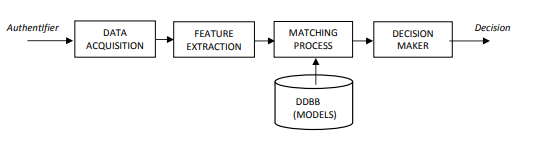
\includegraphics[]{recognition_scheme.png}}
	\caption{Generalna šema generičkog biometrijskog sistema za prepoznavanje.}
	\label{fig:scheme}
\end{figure}

\begin{enumerate}
    \item \textbf{Uzimanje uzorka}: Pravi se uzorak uz pomoć sistema sticanja posebne namene. Ova faza je najosetljivija zbog činjenice da većina algoritama za prepoznavanje zavise od kvaliteta karakteristika uzoraka. Stoga, ako je moguće, kvalitet će se proveravati. Ako je uzorak lošeg kvaliteta, proces će se ponoviti. Takođe je bitno zabeležiti i dovoljan broj uzoraka kako bi se ostvarila visoka robusnost sistema.
    \item \textbf{Ekstrakcija}: Izvlače se jedinstveni podaci koji mogu da se pronađu u uzorku i pravi se šablon.
    \item \textbf{Poređenje}: Izmereni parametri iz prethodnog koraka se koriste za izgradnju modela zadatog korisnika. U slučaju identifikacije, novonastali model se upoređuje sa svim šablonima iz baze podataka, dok se prilikom verifikacije upoređuje samo sa jednim.
    \item \textbf{Odluka}: Sistem odlučuje da li je skup osobina prikupljenih iz uzorka pogodak ili promašaj.
    
    
    
\end{enumerate}

\newpage

\section{Prepoznavanje lica}

Prepoznavanje lica je jedan od metoda biometrijske identifikacije koji najviše obećavaju zato što je to najprirodniji način za prepoznavanje identiteta među ljudskim bićima. Ljudska lica predstavljaju jedan od najčešćih vizuelnih šablona u našoj okolini. Stoga, uobičajeno je za ljude da identifikuju nekoga po njegovom licu, dok bi bilo nemoguće za njih da to urade po otisku prsta, dužici, mrežnjači, čak i po ličnoj karti zbog postojanja velikog broja jezika, čak sa različitim karakterima, širom sveta (Figura \ref{fig:card}). 

\begin{figure}[h!]
	\centerline{
\includegraphics[]{card.png
 }}
	\caption{Lična karta neke osobe. Možemo primetiti da bi zapadnjaci mogli da identifikuju osobu na osnovu slike, ali ne i teksta.}
	\label{fig:card}
\end{figure}

\subsection{Prednosti u odnosu na druge biometrijske osobine}

Jedna od najvećih prednosti je visoka društvena prihvaćenost korisnika jer ne sadrži kriminalne predrasude povezane sa drugim biometrijskim osobinama, poput otiska prstiju. Iako je ova tehnologija uglavnom adaptirana za aplikacije sa kooperativnim korisnicima, interakcija sa korisnicima nije uvek obavezna. Ovaj poslednji aspekt is veoma značajan za primenu u aplikacijama za nadzor na mestima poput aerodroma, železničkim stanicama, visoko obezbeđenim prostorima... Takođe pored identiteta lice prenosi i emocije osobe, kao i biološke informacije (pol, etničku pripadnost, starost...). 


\subsection{Crte lica}

Lice se sastoji od čela, obrva, očiju, nosa, usta, obraza i brade. Antropometrijska istraživanja su pokušala da okarakterišu dimenzije lica bazirane na skupu anatomski značajnih tačaka. Antropometrijske veličine se koriste za istraživanje rasta šablona kod ljudi kao i razumevanje kako se karakteristike lica odnose na pol i etničku pripadnost. Forenzičari su koristili ove tačke kako bi identifikovali lica sa slika. Međutim ove veličine se ne koriste previše u sistemima za automatsko prepoznavanje lica zbog njihovih nedostataka posebnosti. Štaviše, izvlačenje ovi tačaka sa slika lošeg kvaliteta može biti izazovno.

\begin{figure}[h!]
	\centerline{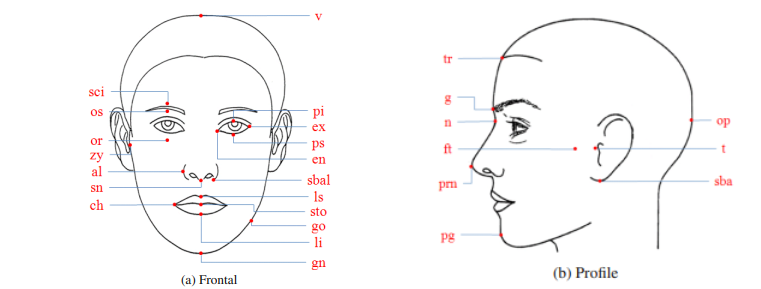
\includegraphics[width=0.8\linewidth]{points.png}}
	\caption{\textbf{Skup anatomski značajnih tačaka}}
	\label{fig:points}
\end{figure}

\newpage

Karakteristike lica se mogu organizovati u tri nivoa:

\begin{itemize}
    \item \textbf{Prvi nivo detalja} se sastoji od grubih karakteristika lica koje su lako uočljive. U njih spadaju npr. geometrija lica i boja kože. Na osnovu njih lako možemo praviti razliku između
    \begin{itemize}
        \item Kratkih, okruglih i dugih, tankih lica
        \item Muških i ženskih lica
        \item Lica ljudi različitih etničkih pripadnosti
    \end{itemize}
    Ove karakteristike se mogu izvući čak i iz slika niskih rezolucija.
    \item \textbf{Drugi nivo detalja} se sastoji od lokalizovanih informacija o licu poput strukture komponenti lica, odnosa izmedju komponenti i preciznog oblika lica. Ove karakteristike su veoma bitne za precizno prepoznavanje lica i one zahtevaju veću rezoluciju slike.
    \item \textbf{Treći nivo detalja} se sastoji od nestruktuiranih, sitnih detalja lica, koji uključuju ožiljke, pege, promena boje kože i mladeža. Ovaj nivo detalja je veoma koristan pri rešavanju veoma problematičnog problema \textit{identičnih blizanaca}.
\end{itemize}

\subsection{Dizajn sistema za prepoznavanje lica}

Tipičan sistem za prepoznavanje lica se sastoji iz tri dela:

\begin{itemize}
    \item Dobijanje slike
    \item Detekcija lica
    \item Poređenje lica
\end{itemize}

Slika lica koja se dobija od senzora može biti kategorisana po  spektralnom opsegu (vidljiv golim okom, infracrveno zračenje, toplotni) korišćenom za slikanje i prirodi tehnike renderovanja slike (2D, 3D i video). Pošto je većina sistema za prepoznavanje lica koriste 2D slike koje su uslikane korišćenjem spektralnog opsega koji je vidljiv golim okom, u nastavku ćemo se fokusirati na procesiranje slika ovog tipa. \textit{Detekcija lica} se odnosi na proces određivanja pozicije lica na slici. Ovaj korak može biti veoma težak u slučaju kada se na slici lice pomeša sa gustom pozadinom. Zbog karakterističnih osobina šablona očiju većina komercijalnih sistema za prepoznavanje lica prvo detektuju oči pa tek posle ostatak lica. Detekcija lica na 3D slikama se smatra jednostavnijem u odnosu na 2D zbog dostupnosti informacija o dubini.

\begin{figure}[h!]
	\centerline{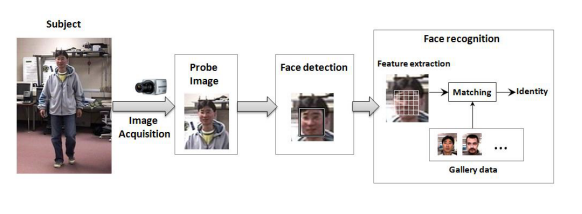
\includegraphics[width=0.8\linewidth]{face_rec_sch.png}}
	\caption{\textbf{Šema procesa prepoznavanja lica}}
	\label{fig:points}
\end{figure}

\subsection{Poređenje lica}

Postoje tri glavna pristupa za poređenje detektovanih lica sa slika:
\begin{itemize}
    \item \textbf{Tehnike zasnovane na izgledu} generišu kompaktnu reprezentaciju cele regije lica u dobijenoj slici mapirajući visokodimenzionalnu sliku lica u niskodimenzionalni podprostor. Ovaj podprostor je definisan skupom reprezentativnih baznih vektora, koji su naučeni tokom treninga nad skupom slika. 
    \item \textbf{Tehnike zasnovane na modelu} grade 2D ili 3D modele lica koji omogućavaju poklapanje lica sa slika u različitim položajima.
    \item \textbf{Tehnike zasnovane na teksturama} pokušavaju da nađu snažne  lokalne karakteristike koje se ne menjaju u zavisnosti od položaja ili osvetljenja.
\end{itemize}
\subsubsection{Tehnike zasnovane na modelu}

Ove tehnike pokušavaju da izvedu reprezentaciju slika lica koja ne zavisi od položaja što bi omogućilo poređenje lica u različitim položajima. Ove šeme obično zahtevaju detekciju par pouzdanih tačaka na licu (ćoškovi očiju, vrh nosa, ćoškovi usana, brada) što dovodi do povećanja kompleksnosti ovih algoritama. Neke od ovih tehnika se mogu koristiti i za generisanje realističnih animacija lica.

Šema \textbf{elastičnog poklapanja grafa grupa} predsavlja lice kao graf čiji su čvorovi pouzdane ili karakteristične tačke lica. Dok je svaki čvor grafa obeležen sa skupom Gaborovih koeficijenata koji karakterišu informacije lokalnih tekstura oko tačaka, svaka grana grafa je obeležena na osnovu rastojanja između odgovarajućih pouzdanih tačaka. Gaborov koeficijent neke tačke na slici se može dobiti  uvijanjem slike uz pomoć kompleksnog 2D Gaborovog filtera centriranog na toj tački. Variranjem orijentacije i frekvencije Gaborovog filtera može se dobiti skup koeficijenata. Korišćenjem pouzdanih tačaka lica omogućeno je pravljenje parcijalnih grafova čak i kada je lice iskrivljeno.

Graf grupa lica (GGL) može biti konstruisan u dve faze od trening skupa slika lica u specifičnim položajima. U prvoj fazi dizajner mora ručno da izabere pouzdane tačke i definiše geometrijsku strukturu grafa slike za jednu ili više početnih slika. Grafovi slika ostalih fotografija iz trening skupa mogu se dobiti poluautomatski, poređenjem novih slika sa modelom grafova (slike koje su već obeležene) na osnovu Gaborovih koeficijenata. Tokom ovog procesa ručna intervencija je obavezna samo ako se pouzdane tačke pogrešno odrede.

\begin{figure}[h!]
	\centerline{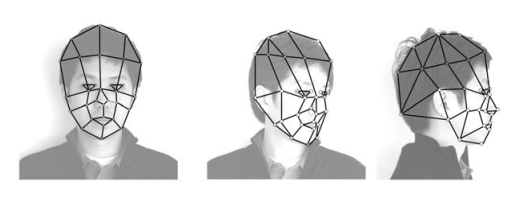
\includegraphics[width=0.8\linewidth]{face_graph.png}}
	\caption{\textbf{Određivanje grafova slike za lice u različitim položajima. Čvorovi su pozicionirani automatski na osnovu poređenja Gaborovih koeficijenata date slike sa onim iz početnog grafa modelovanog od strane dizajnera. }}
	\label{fig:face_graph}
\end{figure}


\newpage

U drugoj fazi GGL se dobija kombinovanjem reprezentativnog skupa individualnih grafova slika u strukturu nalik steku. Tako je svaki čvor u grafu lica  obeležen skupom Gaborovih koeficijenata koji predstavljaju lokalnu varijaciju u odgovarajućoj pouzdanoj tački. Skup Gaborovih koeficijenata koji odgovaraju istoj pouzdanoj tački se nazivaju \textit{grupa}. Na primer, grupa oka može da sadrži  koeficijente otvorenog, zatvorenog, muškog, ženskog... Grane su obeležene na osnovu prosečnog rastojanja između odgovarajućih čvorova u trening skupu.
Kada imamo graf lica, pouzdane tačke za nove slike lica se mogu naći maksimizovanjem sličnosti između grafa koji odgovara datoj slici i grafa identičnog položaja. Ovaj proces se naziva \textit{Elastično poklapanje grafa grupa} i sastoji se od sledeća tri koraka:
\begin{itemize}
    \item Pronalaženje približne pozicije lica grubim skeniranjem slike sa zgusnutim GGL-om. Ovo se postiže određivanjem Gaborovih koeficijenata u određenim tačkama slike i njihovim upoređivanjem sa koeficijentima u zgusnutom GGL-u uzimajući u obzir geometrijsku strukturu GGL-a.
    \item Prečistiti poziciju i veličinu lica ponovnim pretraživanjem slike sa potpunim GGL-om, čija veličina i odnos širine i dužine sistemski variraju. Pri poređenju sličnosti između Gaborovih koeficijenata date slike i koeficijenata GGL-a, samo su razmatrani oni koeficijenti koji se najviše poklapaju.
    \item Precizno određivanje pouzdanih tačaka pomeranjem svih čvorova lokalno i relativno u odnosu na druge u cilju optimizovanja sličnosti grafa u daljem procesu.
\end{itemize}

Rezultat ovog algoritma je slika grafa koji najbolje predstavlja datu sliku.

\begin{figure}[h!]
	\centerline{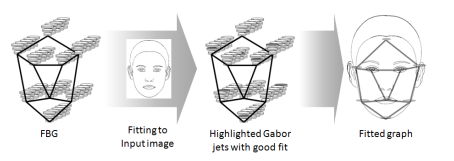
\includegraphics[width=0.8\linewidth]{GGL.png}}
	\caption{\textbf{Graf grupa lica}}
	\label{fig:ggl}
\end{figure}

\newpage

\subsection{Najčešće primene}
\subsubsection{Kontrola pristupa}
S obzirom da većina uređaja danas ima ugrađenu kameru korišćenje tehnologija za prepoznavanje lica je pristupačnija i zbog svoje lakoće korišćenja  u odnosu na šifre predstavlja očigledan izbor. Najpoznatiji sistem za kontrolu pristupa je "\textit{Face ID}" od kompanije Apple.  
\subsubsection{Obezbeđenje privatnih objekata}
Činjenica da računari danas mogu precizno da prepoznaju individualce predstavlja mnoštvo mogućnosti za sigurnosti sektor zbog mogućnosti identifikacije neovlašćenih pristupa lokacijama. Poznato je da IP kamere danas mogu biti opremljene sa softverom za prepoznavanje lica. Uz pomoć belih i crnih lista za specifične lokacije može se implementirati detekcija opasnosti i upada.
\subsubsection{Granični prelazi}
Na graničnim prelazima sve više i više se koriste ovi sistemi za automatsko dozvoljavanje prolaza. Kontrola je povezana sa bazama podataka poput \textit{Intepolove "Facial Identification"  metode}, kako bi identifikovala potencijalno opasne individualce.
\subsubsection{Bankovni sistemi i bankomati}
U većini banaka, njihovi korisnici mogu da omoguće prepoznavanje lica kao dodatan bezbednosni faktor za pristup njihovim nalozima ili pri izvršavanju transakcija.


\subsection{Statistika i zanimljive činjenice}
\begin{enumerate}
    \item \textbf{Sistem za prepoznavanje lica može postići i do 99.97\% preciznosti}. \cite{G3} 
    \break Međutim, ovo je moguće postići samo u idealnim okolnostima (osvetljenje je dobro i konstantno, osoba gleda direktno u kameru i nalazi se blizu nje...). Iz ovog razloga stopa preciznosti je obično oko 90\%. Jedan od glavnih razloga ove razlike od blizu 10\% je što osoba ne gleda direktno u kameru.
    \item \textbf{Šansa da neko drugi otključa vaš telefon preko Face ID je jedan u milion}. \cite{G4}
    \break Kada su telefoni u pitanju, statistike pokazuju da je prepoznavanje lica 20 puta sigurnije od identifikacija zasnovanih na otisku prsta.
    \item \textbf{72\% hotela će verovatno investirati u tehnologije za prepoznavanje lica do 2025.} \cite{G5}
    \break Verovatno nije prva industrija koja bi pala na pamet, ali nije retko da hoteli koriste tehnologije za prepoznavanje lica. Na primer, u Kini možete da se prijavite na recepciji pomoću računara koji vam skenira lice. Takođe prepoznavanje lica zamenjuje ključeve, plaćanje bez kontakta i nadzor gostiju.
    \item \textbf{Market prepoznavanja lica je proizveo 3.8 milijardi dolara samo u 2020.} \cite{G6}
    \break Sa sektorima za odbranu, bezbednost i sličnim organizacijama koje investiraju sve više i više, ovo i nije toliko iznenađujuće. Štaviše, eksperti očekuju da će market dostići i do 8.5 milijardi dolara do 2025, što znači da će se duplirati u odnosu na trenutnu vrednost.
    \item \begin{flushleft} \textbf{U Kini možete "platiti osmehom" u KFC-u.}  \cite{G7}\end{flushleft} 
    Mnogi od nas su se već navikli na život bez gotovine plaćajući karticama ili čak telefonima. Ipak \textit{Alibaba} se čini dva koraka ispred. Njihova najnovija tehnologija omogućava da 3D kamera skerina lice kupca i automatski skine svotu sa njihovog Alipay novčanika.
    \item \textbf{U Americi, tehnologija za prepoznavanje lica ima stopu odobrenja od 83\%. \cite{G8}} 
    \break Držanje opasnih ljudi van prostora škola i pronalaženje nestalih osoba su neke od glavnih argumenata osoba koje podržavaju ovu tehnologiju. Aerodromi u Americi već uveliko koriste sisteme za prepoznavanje lica.
    \item \begin{flushleft}  \textbf{Belgija i Luksenburg su zabranili korišćenje.} \cite{G9} \end{flushleft} 
    Ovo su jedine dve države koje su zabranile korišćenje, iako su Belgijske kriminalističke službe koristile prepoznavanje lica - ilegalno. U septembru 2021, policija je poricala optužbe, ali mesec dana kasnije ministar unutrašnjih poslova je priznao da je tehnologija korišćena 100 do 500 puta.
   
    
\end{enumerate}

\section{Zaključak}
Tehnologija prepoznavanja lica konačno dostiže zavidan napredak i brz rast u praktičnim primenama. Velika količina istraživačkog truda svuda oko sveta biva primenjena na poboljšanje preciznosti i proširenje mogućnosti u ovom biometrijskom domenu. Iako već postoji ogroman broj primena, iz dana u dan zbog novih okolnosti ljudi nalaze još više primena. U bliskoj budućnosti možemo očekivati još veći broj uređaja koji koriste ovaj vid sigurnosnih protokola. 





\newpage
\begin{thebibliography}{9}

    \bibitem{G1} 
    Introduction to biometrics Anil K. Jain, Arun A. Ross, Karthik Nandakumar

    \bibitem{G2} 
    Face Recognition by means of advanced contributions in machine learning, Ph.D. thesis, Virginia Espinosa Duro
    
    \bibitem{G3} 
    Center For Strategic \& International Studies: How Accurate are Facial Recognition Systems – and Why Does It Matter?

    \bibitem{G4} 
    9TO5Mac - In-screen Touch ID potentially signals a backward step ahead

    \bibitem{G5}
    Forbes - Improving User Experiences In The Hospitality Industry

    \bibitem{G6}
    Comparitech - Facial recognition report highlights growing, variable global market

    \bibitem{G7}
    TechCrunch - "Smile to pay"

    \bibitem{G8}
    NetChoice - Americans Want Facial Recognition Use By Law Enforcement Improved, But Not Banned

    \bibitem{G9}
    The Brussels Times

    
    
    
    
\end{thebibliography}

\end{document}
